\documentclass[spec, och, labwork]{shiza}
% параметр - тип обучения - одно из значений:
%    spec     - специальность
%    bachelor - бакалавриат (по умолчанию)
%    master   - магистратура
% параметр - форма обучения - одно из значений:
%    och   - очное (по умолчанию)
%    zaoch - заочное
% параметр - тип работы - одно из значений:
%    referat    - реферат
%    coursework - курсовая работа (по умолчанию)
%    diploma    - дипломная работа
%    pract      - отчет по практике
% параметр - включение шрифта
%    times    - включение шрифта Times New Roman (если установлен)
%               по умолчанию выключен
\usepackage{subfigure}
\usepackage{tikz,pgfplots}
\pgfplotsset{compat=1.5}
\usepackage{float}

%\usepackage{titlesec}
\setcounter{secnumdepth}{4}
%\titleformat{\paragraph}
%{\normalfont\normalsize}{\theparagraph}{1em}{}
%\titlespacing*{\paragraph}
%{35.5pt}{3.25ex plus 1ex minus .2ex}{1.5ex plus .2ex}

\titleformat{\paragraph}[block]
{\hspace{1.25cm}\normalfont}
{\theparagraph}{1ex}{}
\titlespacing{\paragraph}
{0cm}{2ex plus 1ex minus .2ex}{.4ex plus.2ex}

% --------------------------------------------------------------------------%


\usepackage[T2A]{fontenc}
\usepackage[utf8]{inputenc}
\usepackage{graphicx}
\graphicspath{ {./images/} }
\usepackage{tempora}

\usepackage[sort,compress]{cite}
\usepackage{amsmath}
\usepackage{amssymb}
\usepackage{amsthm}
\usepackage{fancyvrb}
\usepackage{listings}
\usepackage{listingsutf8}
\usepackage{longtable}
\usepackage{array}
\usepackage[english,russian]{babel}

% \usepackage[colorlinks=true]{hyperref}
\usepackage{url}

\usepackage{underscore}
\usepackage{setspace}
\usepackage{indentfirst} 
\usepackage{mathtools}
\usepackage{amsfonts}
\usepackage{enumitem}
\usepackage{tikz}
\usepackage{minted}

\newcommand{\eqdef}{\stackrel {\rm def}{=}}
\newcommand{\specialcell}[2][c]{%
\begin{tabular}[#1]{@{}c@{}}#2\end{tabular}}

\renewcommand\theFancyVerbLine{\small\arabic{FancyVerbLine}}

\newtheorem{lem}{Лемма}

\begin{document}

% Кафедра (в родительном падеже)
\chair{}

% Тема работы
\title{Преобразователи кодов}

% Курс
\course{3}

% Группа
\group{331}

% Факультет (в родительном падеже) (по умолчанию "факультета КНиИТ")
\department{факультета КНиИТ}

% Специальность/направление код - наименование
%\napravlenie{09.03.04 "--- Программная инженерия}
%\napravlenie{010500 "--- Математическое обеспечение и администрирование информационных систем}
%\napravlenie{230100 "--- Информатика и вычислительная техника}
%\napravlenie{231000 "--- Программная инженерия}
\napravlenie{10.05.01 "--- Компьютерная безопасность}

% Для студентки. Для работы студента следующая команда не нужна.
% \studenttitle{Студентки}

% Фамилия, имя, отчество в родительном падеже
\author{Стаина Романа Игоревича и Токарева Никиты Сергеевича}

% Заведующий кафедрой
% \chtitle{} % степень, звание
% \chname{}

%Научный руководитель (для реферата преподаватель проверяющий работу)
\satitle{аспирант} %должность, степень, звание
\saname{А. А. Мартышкин}

% Руководитель практики от организации (только для практики,
% для остальных типов работ не используется)
% \patitle{к.ф.-м.н.}
% \paname{С.~В.~Миронов}

% Семестр (только для практики, для остальных
% типов работ не используется)
%\term{8}

% Наименование практики (только для практики, для остальных
% типов работ не используется)
%\practtype{преддипломная}

% Продолжительность практики (количество недель) (только для практики,
% для остальных типов работ не используется)
%\duration{4}

% Даты начала и окончания практики (только для практики, для остальных
% типов работ не используется)
%\practStart{30.04.2019}
%\practFinish{27.05.2019}

% Год выполнения отчета
\date{2022}

\maketitle

% Включение нумерации рисунков, формул и таблиц по разделам
% (по умолчанию - нумерация сквозная)
% (допускается оба вида нумерации)
% \secNumbering

%-------------------------------------------------------------------------------

% \tableofcontents

\section{Цель работы:}

Ознакомление с основными характеристиками и испытание 
интегральных преобразователей кодов (дешифратора, шифратора, демультиплексора 
и мультиплексора).

\textbf{Задание 1.}

Построим схему дешифратора DC:

\begin{figure}[H]
    \centering
    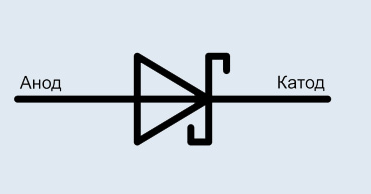
\includegraphics[width=0.8\textwidth]{pic2/1.png}
    \caption{}
\end{figure}

По результатам моделирования составим и заполним таблицу переключений 
функций $Y_i=(A_iB_iC_i;G_i)$ на выходах дешифратора $DC ~3\text{x}8$.

\begin{table}[h]
    \begin{center}
    \begin{tabular}{|l|l|l|l|l|l|l|l|l|}
    \hline
          & $X_0$ & $X_1$ & $X_2$ & $X_3$ & $X_4$ & $X_5$ & $X_6$ & $X_7$ \\ \hline
    $A_i$ &       & 1     &       & 1     &       & 1     &       & 1     \\ \hline
    $B_i$ &       &       & 1     & 1     &       &       & 1     & 1     \\ \hline
    $C_i$ &       &       &       &       & 1     & 1     & 1     & 1     \\ \hline
    \end{tabular}
\end{center}
\end{table}


\textbf{Задание 2.}

Построим схему шифратора $CD$:


\begin{center}$y=(ab+\urcorner c)(\urcorner a+\urcorner b+c)(a+b+c)$\end{center}

\begin{figure}[H]
    \centering
    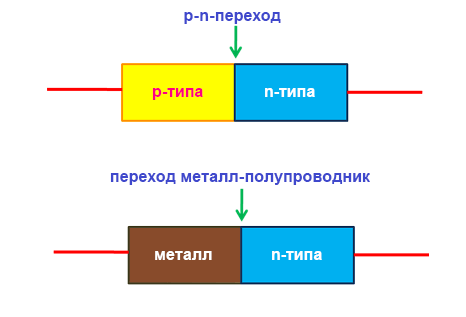
\includegraphics[width=0.8\textwidth]{pic2/2.png}
    \caption{}
\end{figure}

По результатам моделирования (по подсвечиванию пробников $X_0,X_1,X_2$ и 
показаниям индикатора $Ind$) составим и заполним таблицу переключений на выходе
шифратора $CD ~8\text{x}3$:

\begin{table}[h]
    \begin{center}
    \begin{tabular}{|l|l|l|l|}
    \hline
          & $A_i$ & $B_i$ & $C_i$ \\ \hline
    $X_0$ &       &       &       \\ \hline
    $X_1$ & 1     &       &       \\ \hline
    $X_2$ &       & 1     &       \\ \hline
    $X_3$ & 1     & 1     &       \\ \hline
    $X_4$ &       &       & 1     \\ \hline
    $X_5$ & 1     &       & 1     \\ \hline
    $X_6$ &       & 1     & 1     \\ \hline
    $X_7$ & 1     & 1     & 1     \\ \hline
    \end{tabular}
    \end{center}
\end{table}

Преобразуем схему дешифратора $DC~3 \text{x}8$ и шифратора $CD~8\text{x}3$ в схему
$DC ~2\text{x}4$ и шифратора $CD~4\text{x}2$, отсоединив провод $C$, подходящий
к дешифратору, и провод $A2$ с выхода шифратора, и составим таблицы переключений
дешифратора 2x4 и шифратора 4x2:

\begin{table}[H]
    \begin{center}
    \begin{tabular}{|l|l|l|l|l|}
    \hline
          & $X_0$ & $X_1$ & $X_2$ & $X_3$ \\ \hline
    $A_i$ &       & 1     &       & 1     \\ \hline
    $B_i$ &       &       & 1     & 1     \\ \hline
    \end{tabular}
    \end{center}
\end{table}

\begin{table}[H]
    \begin{center}
    \begin{tabular}{|l|l|l|}
    \hline
          & $A_i$ & $B_i$ \\ \hline
    $X_0$ &       &       \\ \hline
    $X_1$ & 1     &       \\ \hline
    $X_2$ &       & 1     \\ \hline
    $X_3$ & 1     & 1     \\ \hline
    \end{tabular}
    \end{center}
\end{table}


\textbf{Задание 3.}

Построим схему демультиплексора $DMS$.

\begin{figure}[H]
    \centering
    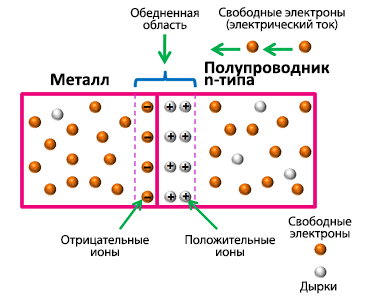
\includegraphics[width=0.8\textwidth]{pic2/3.png}
    \caption{}
\end{figure}

Временные диаграммы входных и выходных сигналов:

\begin{figure}[H]
    \centering
    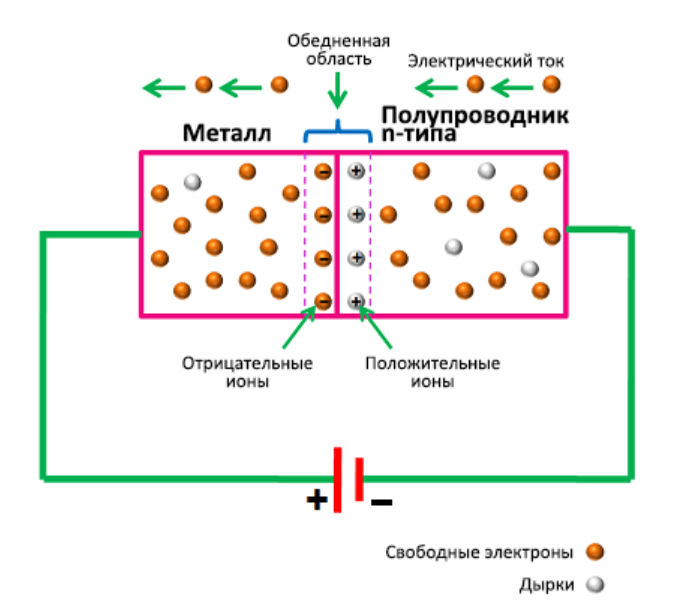
\includegraphics[width=0.8\textwidth]{pic2/4.png}
    \caption{}
\end{figure}

\textbf{Задание 4.}

Построим схему мультиплексора $MS$.

\begin{figure}[H]
    \centering
    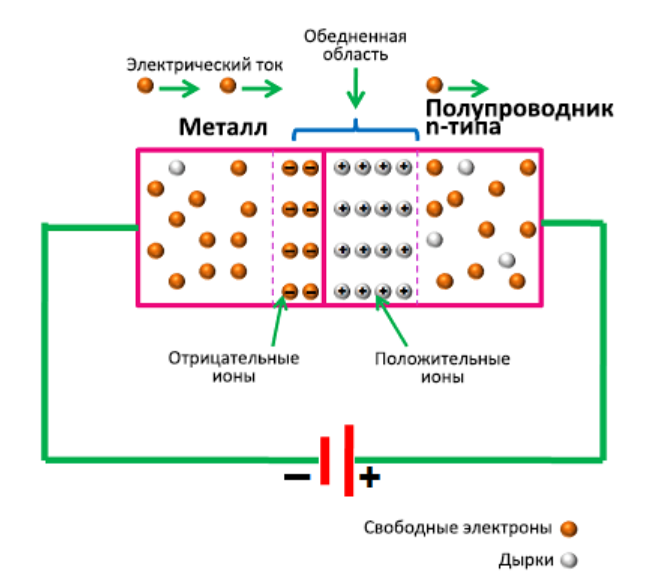
\includegraphics[width=0.8\textwidth]{pic2/5.png}
    \caption{}
\end{figure}

Установим с помощью ключей $A,B,C$ адресный код $110_2 = 6_10$

Временные диаграммы входных данных сигналов $D_0,D_1,...,D_7$ и выходного
сигнала $Y$ мультиплексора:

\begin{figure}[H]
    \centering
    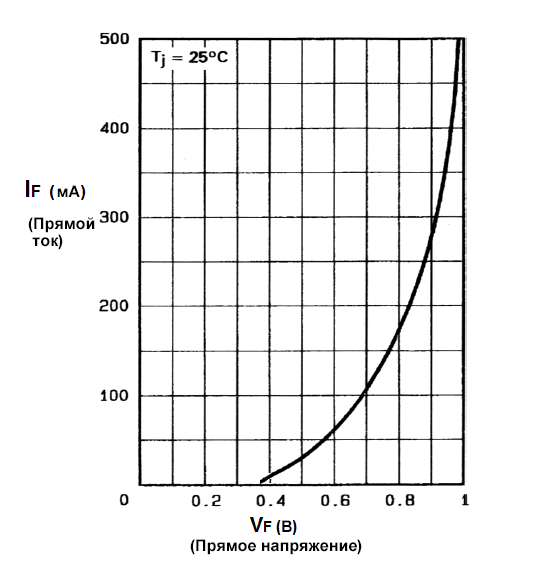
\includegraphics[width=0.8\textwidth]{pic2/6.png}
    \caption{}
\end{figure}


\textbf{Вывод:} в ходе лабораторной работы мы ознакомились с основными характеристиками
интегральных преобразователей кодов: дешифратора, шифратора, демультиплексора и 
мультиплексора. Также ознакомились с их практическим применением.


\section{Тестовые задания к работе 30:}

\begin{enumerate}
        \item Укажите \textbf{задачи}:
        
        \begin{enumerate}
            \item[a)] для мультиплексирования данных и адресной логики в запоминающих
            устройствах, а также для преобразования двоично-десятичного кода в 
            десятичный с целью управления индикаторными и печатающими устройствами;

            \item[б)] для преобразования десятичных чисел в двоичные или двоично-десятичный
            код, например в микрокалькуляторах, в которых нажатие десятичных
            клавишей соответствует генерации соответствующего двоичного кода;

            \item[в)] для хранения и преобразования многоразрядных двоичных чисел;
            
            \item[г)] для коммутации в заданном порядке сигналов, поступающих с
            нескольких входных шин на одну выходную;

            \item[д)] для распределения в требуемой последовательности по нескольким 
            выходам сигналов с одного информационного входа, в частности для передачи 
            информации по одной линии от нескольких установленных на ней датчиков.
        \end{enumerate}
        
        При решении которых используется:
        \begin{enumerate}
            \item[1.] шифратор;
            \item[2.] дешифратор;
            \item[3.] мультиплексор;
            \item[4.] демультиплексор.
        \end{enumerate}

        Ответ: 1 - б, 2 - а, 3 - г, 4 - д.

        \item Укажите, с \textbf{какого разряда} бинарного слова генератора $XWG$ будет
        передаваться информация на выход мультиплексора 8х3 при адресном коде 100
        на его входе:
        
        Ответ: 7.

        \item Укажите число \textbf{выходов} дешифратора при трех информационных входах:

        Ответ: 8.
        
        \item Укажите назначение\textbf{стробирующих} входов в преобразователях кодов: 

        Ответ: для увеличения числа коммутируемых информационных входов, а также
        для блокирования работы преобразователей.

        \item Укажите, в каком \textbf{преобразователе} выбор выхода по его номеру (адресу)
        осуществляется с помощью двоичного кода:

        Ответ: в мультиплексоре.
        
        \item Укажите \textbf{число выходов} у шифратора при четырех информационных
        входах:

        Ответ: 2.
        
        \item Укажите, какой из приведенных преобразователей кодов выпускается промышленностью
        только в \textbf{составе других устройств}:

        Ответ: мультиплексор.

\end{enumerate}

\end{document}